%%part6
\MinParskip{}

\section{Sensitivity Analysis}

We chose California to test the sensitivity of our model. We selected two indicators, regional industrial structure and limit magnitude, which are cost-based and benefit-based, to test the sensitivity of our model.

1. Regional industrial structure

California's regional industrial structure is 0.2229. We have studied the change of California's light-light intensity when the regional industrial structure changes from 0.20 to 0.25. From the chart, we can see that the night-light intensity of California is 0.59146 at this time. When the regional industrial structure changes to 0.20, the night-light intensity decreases to 0.58000, and the relative change rate is 1.94\%. The relative change rate from 0.2229 to 0.20 is 10.3\%, and the ratio of the two relative change rates is 0.188. When the regional industrial structure changes to 0.25, the night-light intensity increases to 0.60490, and the relative change rate is 2.27\%. The relative change rate from 0.2229 to 0.25 is 12.2\%, and the ratio of the two relative change rates is 0.186. Therefore, we can see that our model will not deviate greatly due to the deviation of the regional industrial structure.

And we can see continuous night-time light intensity changes with regional industrial structure as the following figure.

2. Limit magnitude

California's limit magnitude is 6. We have studied the change of California's light-light intensity when the limit magnitude changes from 5 to 7. From the chart, we can see that the night-light intensity of California is 0.59146 at this time. When the limit magnitude changes to 5, the night-light intensity decreases to 0.59908, and the relative change rate is 1.29\%. The relative change rate from 6 to 5 is 16.7\%, and the ratio of the two relative change rates is 0.08. When the limit magnitude changes to 7, the night-light intensity increases to 0.58320, and the relative change rate is 1.40\%. The relative change rate from 6 to 7 is 16.7\%, and the ratio of the two relative change rates is 0.08. Therefore, we can see that our model will not have a large deviation due to the deviation of Limit Magnitude.

And we can see continuous night-time light intensity changes with limit magnitude as the following figure.
\begin{figure}[H]\centering
    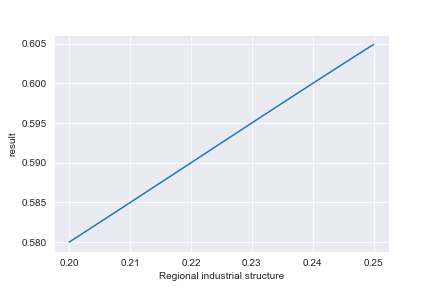
\includegraphics[width=0.88\textwidth]{figures/Regional_industrial_structure.png}
    \caption{Night-time Light Intensity Changes With Regional Industrial Structure} \label{fig:figure7}
\end{figure}

\begin{figure}[H]\centering
    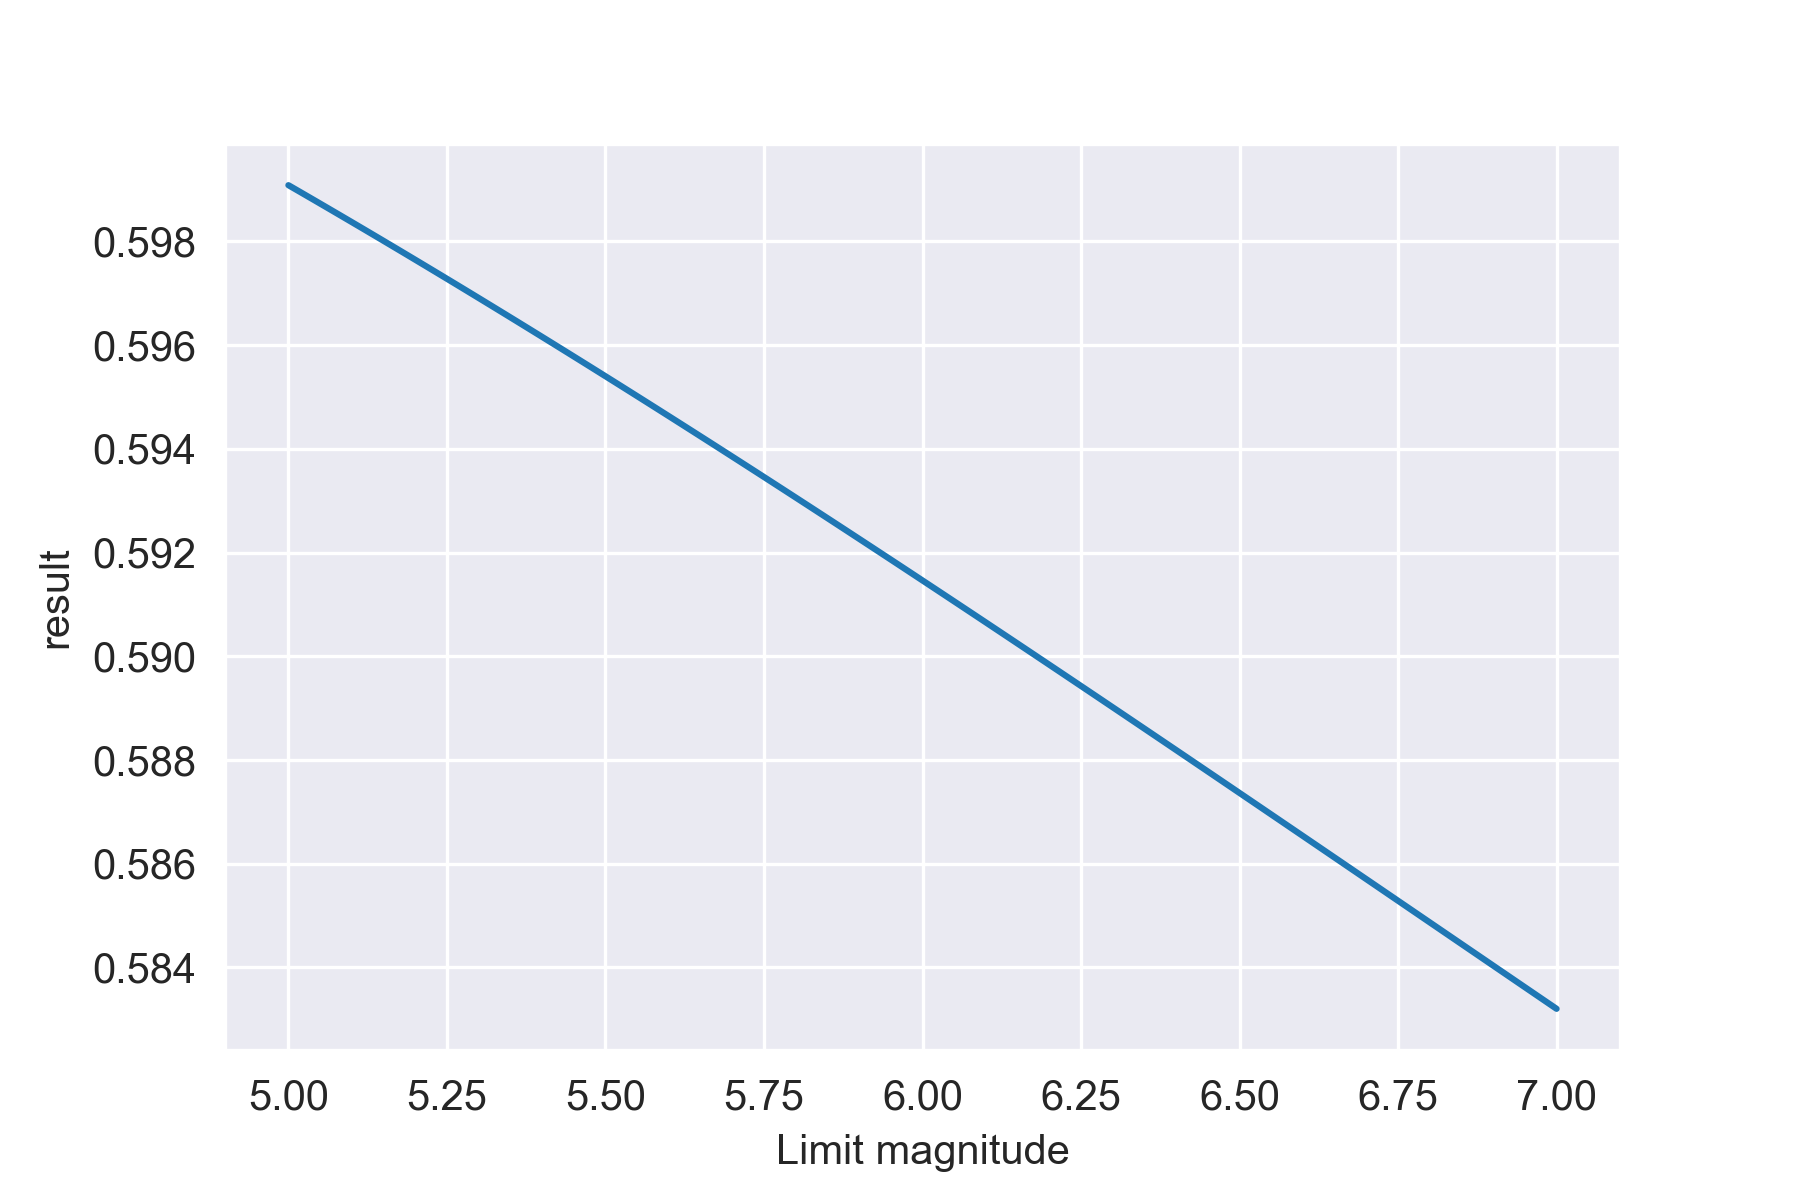
\includegraphics[width=0.88\textwidth]{figures/Limit_magnitude.png}
    \caption{Night-time Light Intensity Changes With Limit Magnitude} \label{fig:figure8}
\end{figure}